%!TEX root = ../aamas11storage.tex
% %%%%%%%%%%%%%%%%%%%%%%%%%%%%%%%%%%%%%%%%%%%%%%%%%%%
\section{Modular Storage Application}\label{sec:introduction}
% %%%%%%%%%%%%%%%%%%%%%%%%%%%%%%%%%%%%%%%%%%%%%%%%%%%

Energy storage enables increasing levels of renewable energy in our electricity system, and the rapidly maturing supply chains for several battery technologies encourages electricity utilities, generators, and customers to consider using large battery systems. 

Consider the example scenario of a smart office building comprising of a set of loads (appliances in the building), some renewable sources (solar panels on the roof and a local wind turbine), and a modular battery system. The building is connected to the main grid, and the economics govern that the grid power consumption of the building be maintained within the range $[p_l:p_h]$. Since there is little control over the demand in the building and certainly no control over the renewable generation, then for some period in the day it is possible that the power consumption of the building will fall outside this range. For instance, if the renewable generation is higher than the demand, then the consumption will be negative. Similarly, if the demand is higher than the renewable generation then the building consumption may rise above $P$. In Figure \ref{fig:usecase} the Building Demand plots the sum of consumption and renewable generation in the building and has this property for the period prior to time $t_1$ and after time $t_2$. While this net building demand is fixed all all practical purposes, we do have full control over the use of the battery system. By suitably ordering the battery system to charge (act as a load) or discharge (act as a generator) at determined rates through this period we may influence the net demand in the building. Figure \ref{fig:usecase} shows how the appropriate battery response (Battery Charge) added to the net building consumption (Building Demand) ensures that the power drawn from the grid (Grid Supply) is maintained within the desired range $[p_l:p_h]$.

\begin{figure}[ht]
\begin{center}
%!TEX root = ../aamas11storage.tex
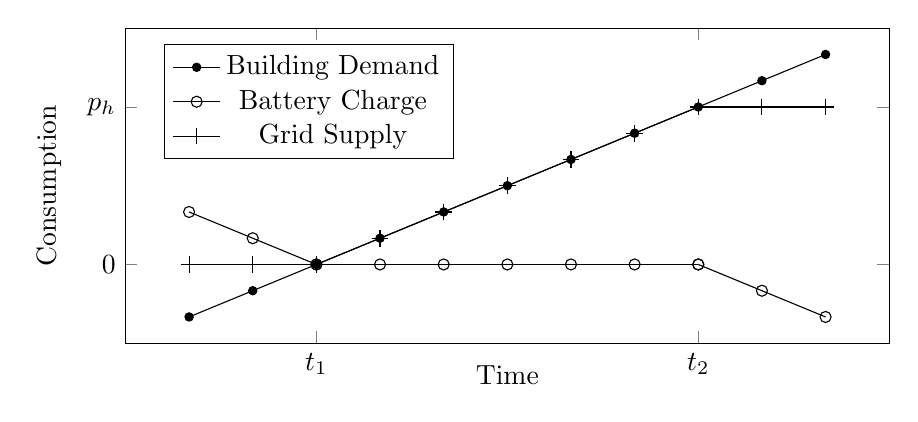
\begin{tikzpicture}

\begin{axis}[
width=0.8\columnwidth,height=4cm,scale only axis,
axis line style={-}, xtick style={-}, ytick style={-},
xlabel=Time,
ylabel=Consumption,
every axis y label/.style={at={(-0.1,0.5)},rotate=90,anchor=center}, 
every axis x label/.style={at={(0.5,-0.1)},anchor=center}, 
%grid=both, grid style={style=densely dotted},
xtick={2,8},
xticklabels={$t_1$,$t_2$},
ytick={0,6},
yticklabels={$0$,$p_h$},
legend style={at={(0.05,0.95)},anchor=north west}
] 

% Draw the Demand-Supply curve
\addplot[-,mark=*,mark size=1.5] expression[domain=0:10,samples=11] {x-2};
\addlegendentry{Building Demand} 

% Draw the Battery curve
\addplot[-,mark=o,mark size=2] expression[forget plot,domain=0:2,samples=3] {2-x}; 
\addplot[-,mark=o,mark size=2] expression[forget plot,domain=2:8,samples=7] {0}; 
\addplot[-,mark=o,mark size=2] expression[domain=8:10,samples=3] {8-x}; 
\addlegendentry{Battery Charge} 

% Draw the Grid supply curve
\addplot[-,mark=+,mark size=3] expression[forget plot,domain=0:2,samples=3] {0}; 
\addplot[-,mark=+,mark size=3] expression[forget plot,domain=2:8,samples=7] {x-2}; 
\addplot[-,mark=+,mark size=3] expression[domain=8:10,samples=3] {6}; 
\addlegendentry{Grid Supply} 
\end{axis} 
\end{tikzpicture} 

\end{center}
\caption{Use case scenario for a modular battery system.}
\label{fig:usecase}
\end{figure}

Large battery systems usually comprise of multiple modules and in many installations these may be controlled independently.  Modules may be operated in synchrony but often there are strategic reasons to keep some modules in a different state to others.  For example, if it is undesirable to change the direction of power flow between charging and discharging too frequently, a subset of modules may be used for each direction until it is necessary to change their roles.  Also, some technologies have specific requirements, such as the zinc-bromine flow battery for which a complete discharge at regular intervals is desirable to ``strip'' the zinc plating and ensure irregularities never have an opportunity to accumulate.  Where they exist these requirements place further constraints on module control.

Given, then, an input signal which is the requested rate of charging and discharging for a large battery installation as a function of time, we would like a control algorithm for the set of component modules that implements the requested rate as the sum over the module rates of charging and discharging.  While hardwired control of the battery response is possible, it is often not ideal since the module chemistry is susceptible to change over time and will often cause the battery system performance to diverge from normal. What is needed is adaptable control that accounts for such drift, and as such, a  machine learning approach may be appropriate. 
%The input signal will be different every day but will have many features that are diurnal or nearly so, due to typical variations of electricity demand and solar and wind energy generation sources, and the repetitive patterns that may be seen over several days of the input signal suggest that a learning algorithm may be appropriate.  Our problem is to develop a method for on-line learning that will result in a useful control regime for a modular battery system, when installed at a new site and provided with an input signal derived from the electricity demand and renewable supply at that site.

\begin{figure*}[ht]
\begin{center}
%!TEX root = ../aamas11storage.tex
\begin{tikzpicture} [level distance=8.0em]
\tikzstyle{planbox}=[draw,text width=11.0em,rectangle split,rectangle split parts=3]
\tikzstyle{goalbox}=[draw,rounded corners=1.25em,minimum height=3em,minimum width=5em]

	
\tikzstyle{level 1}=[sibling distance=13.0em] 
\tikzstyle{level 2}=[level distance=7.0em] 

\node[goalbox,solid] {$G($r,k,s$)$}
	child {node[planbox] {$SetCharge$ 
			\nodepart{second} $\psi:satisfies(r,k,s,C),$\\$k>0$
			\nodepart{third} $set(k,C)$
		}
		child {node[goalbox] {$G($r,k-1,s'$)$}}
	}
	child {node[planbox] {$SetDischarge$ \nodepart{second}
			\nodepart{second} $\psi:satisfies(r,k,s,D),$\\$k>0$
			\nodepart{third} $set(k,D)$
		}
		child {node[goalbox] {$G($r,k-1,s'$)$}}
	}
	child {node[planbox] {$SetNotUsed$ \nodepart{second}
			\nodepart{second} $\psi:satisfies(r,k,s,N),$\\$k>0$
			\nodepart{third} $set(k,N)$
		}
		child {node[goalbox] {$G($r,k-1,s'$)$}}
	}
	child {node[planbox] {$Execute$ 
			\nodepart{second} $\psi:k==0$
			\nodepart{third} $operate()$ \\$evaluate()$
		}
	}
;

\end{tikzpicture}



\end{center}
\caption{Goal-plan hierarchy for the battery system with $k$ modules.}
\label{fig:gptree}
\end{figure*}


% %%%%%%%%%%%%%%%%%%%%%%%%%%%%%%%%%%%%%%%%%%%%%%%%%%%
\subsection{System Design}\label{subsec:design}
% %%%%%%%%%%%%%%%%%%%%%%%%%%%%%%%%%%%%%%%%%%%%%%%%%%%

Figure \ref{fig:gptree} shows a BDI controller for a battery system with $k$ modules. At the beginning of each period of deliberation, the environment posts the top-level goal $G(r,k,s)$. The controller then responds by operating the battery system for that period in a suitable operational state that resolves the goal. Here $r$ specifies the desired response from the battery system and lies in the normalised range $[-1.0:+1.0]$ where $-1.0$ indicates a maximum discharge rate (where all modules are discharging) and $+1.0$ indicates a maximum charge rate (where all modules are charging). The parameter $s$ represents the current state of the battery system, and is derived from sensor readings of each modules current charge and operational state, and $k$ is initially set to the number of modules in the system. 

The resolution of the battery system decides how closely it can match the desired response and is determined by the number of modules $n$. For simplicity, we will assume homogeneous capacity of the modules (but with possibly different chemical properties and constraints), such that each module has a normalised capacity $c$ and $c*n=1.0$. Each module in turn may be configured in one of three states: charging (i.e $+c$), discharging (i.e. $-c$) or not in use (i.e. $0$). The sum of these values gives the net response of the system. By appropriately setting each modules operational state then, the response of the battery system may be adjusted in the range $[-1.0:+1.0]$ in steps of $\pm c$.

The BDI controller works by recursively setting the operational state of each module using the respective $Set*$ plans, and then finally executing the resulting battery configuration for one period and evaluating the result using the $Execute$ plan. The execution therefore always consists of the selection of $k$ high level $Set*$ plans followed by the $Execute$ leaf plan. Using the BDI learning framework from \cite{Singh:RAS10} the pass/fail result is then recorded in the chain of active plans for that period. By training over the outcomes of plan selections in each situation, the system over time learns correct plan selection at each recursive level for the set of possible top-level requests. Each plan in the goal-plan hierarchy is further explained below:

$SetCharge$: Set the operational state of module $k$ to {\em Charge} (i.e $+c$) for this period. The plan first checks that the internal constraints of module $k>0$ will not be violated by this operation. If a violation is expected, then the plan is discarded, otherwise the state is updated and Goal $G$ reposted for module $k-1$.

$SetDischarge$: Set the operational state of module $k$ to {\em Discharge} (i.e $-c$) for this period. The plan first checks that the internal constraints of module $k>0$ will not be violated by this operation. If a violation is expected, then the plan is discarded, otherwise the state is updated and Goal $G$ reposted for module $k-1$.

$SetNotUsed$: Set the operational state of module $k$ to {\em NotUsed} (i.e $0$). This means that the module will remain disconnected from use for this period. The plan first checks that the internal constraints of module $k>0$ will not be violated by this operation. If a violation is expected, then the plan is discarded, otherwise the state is updated and the Goal $G$ reposted for module $k-1$.

$Execute$: The leaf plan that actually performs the operations on the battery modules. The plan executes only when $k=0$ which implies that all modules have been configured. All battery modules are then operated simultaneously for this period according to their assigned states. At the end of the period, the plan will evaluate the net battery response against the request. From a learning perspective, the battery response is deemed successful only if it was within tolerance of the desired response, otherwise it is deemed failed.


A $Set*$ plan may be discarded from consideration if the respective constraints for module $k$ are not satisfied for that period. For instance, plan $SetCharge$ may be discarded because module $k$ is only allowed to change charge directions once every four periods say, and charging it in this period will violate that constraint. Similarly, plan $SetDischarge$ may be discarded because the module may already be discharged and further discharge is not possible. Finally, plan $SetNotUsed$ may be discarded because setting module $k$ to this state would imply that the request will become unserviceable regardless of how the as-yet-unassigned modules are configured. For instance, a request of $+1.0$ is only serviceable when all modules are configured to charge. If one of the modules were to not charge (it may already be fully charged so further charging is not possible), then any further configuration is pointless because the response is bound to fail.

Since constraint checking is performed in the context condition of the plan i.e. prior to taking any action in the plan body, then BDI failure recovery may be employed to select different $Set*$ plans until all internal constraints are satisfied. Note that failure recovery is not allowed for the $Execute$ plan because it runs for a full period and that is the limit for the decision making. In other words, only one try is allowed per period. So functionally, the $Execute$ plan must always succeed, even though the evaluation against the goal (for learning purposes) may differ.

Finally, the system only learns a response to the immediate request i.e. how to resolve the top level goal. It does not learn any temporal relationship in the sequence of top level goals. For instance, the input signal may have some diurnal or seasonal pattern, however the proposed system does not attempt to learn this pattern. This is perfectly acceptable since then time-scale for decision making by the controller (in the order of seconds) is very short compared to the frequency of the pattern.

% %%%%%%%%%%%%%%%%%%%%%%%%%%%%%%%%%%%%%%%%%%%%%%%%%%%
\subsection{Experimental Setup}\label{experiments}
% %%%%%%%%%%%%%%%%%%%%%%%%%%%%%%%%%%%%%%%%%%%%%%%%%%%

Modules=5, Period=1minute, Tolerance=0. Check all run parameters.

% %%%%%%%%%%%%%%%%%%%%%%%%%%%%%%%%%%%%%%%%%%%%%%%%%%%
\subsection{Analysis}\label{analysis}
% %%%%%%%%%%%%%%%%%%%%%%%%%%%%%%%%%%%%%%%%%%%%%%%%%%%

%The system is (purposely) similar in design to the Towers of Hanoi problem of \cite{Singh:RAS10}. In some respects, it is simpler because the solutions are always at recursive depth $k$. Moreover, the non-leaf $Set*$ plans do not have side-effects when they fail and leave the initial state unaltered. Finally, a solution always consists of a single $Execute$ action whereas in the Hanoi problem it consists of possibly several $Move$ actions\footnote{One point of difference is that this is not a universal library where a solution can always be found. For some requests, no solution will be possible given the internal state of the modules.}.

%Nonetheless, the problem captures a real world problem where it is not straightforward to hand-craft a functional hierarchy and where learning is justified. We do not have a solution to begin with. Then, the size of the problem is still significant - the flow battery in CSIRO Newcastle has $10$ internal modules, so with three possible module states that represents $3^{10}=59049$ possible configurations for a given request. Finally, it offers a realistic scenario for re-learning a solution due to significant changes in the environment. For instance, if an internal module were to fail and had to be replaced, then prior learning may no longer work effectively, and the system will have to adjust and re-learn it's response based on the new characteristics of the updated module.
